\chapter{Implementation}
\label{chap:implementation}

% rename chapter to Use cases

% first paragraph:
% architecture was described
% now we show how to use it
% two examples
% one subsection about aggregations
% one subsection about anomaly detection

Aggregations

In our project we use two types of aggregations: user-based and application-based.
Figure~\ref{fig:user_based_aggregations} represents the table of user-based aggregations.
Each of these aggregations is calculated with different granularities: hourly, daily, weekly and monthly.

\begin{figure}
  \centering
  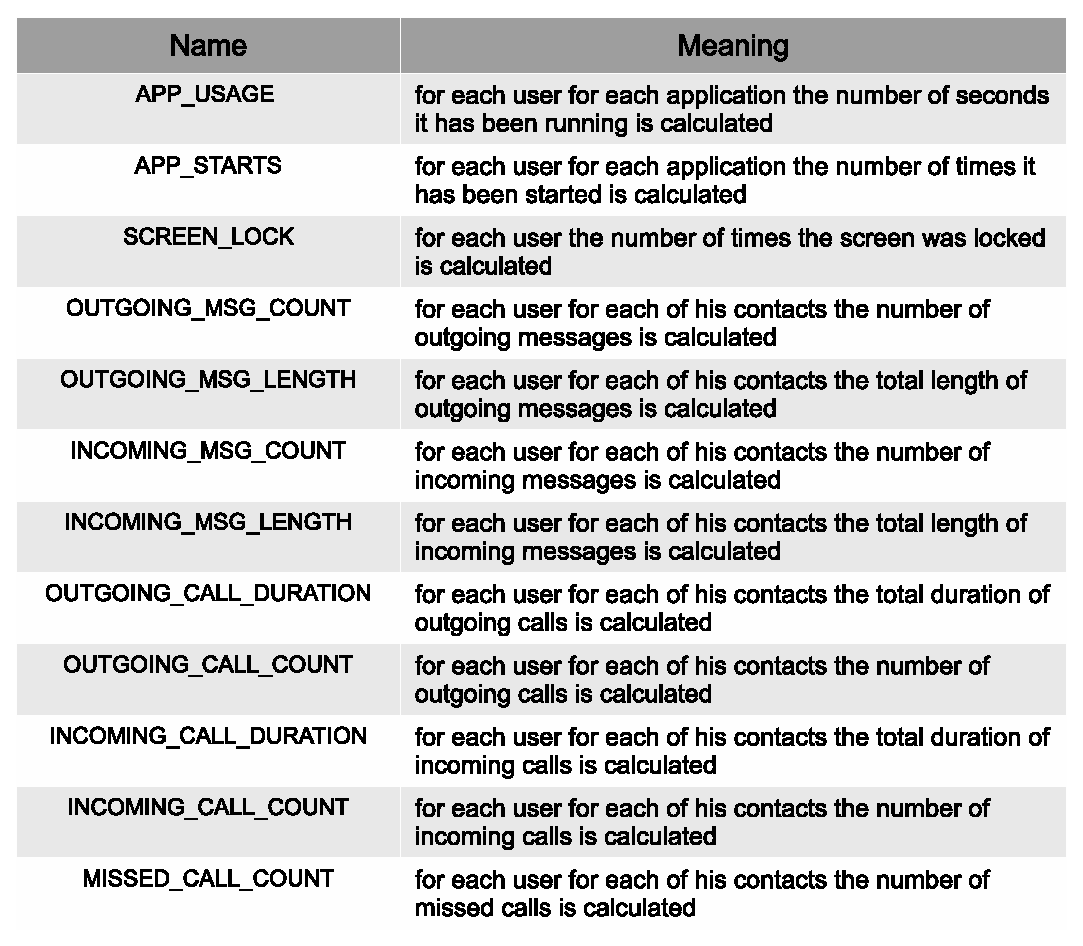
\includegraphics [width=1.0\textwidth]{images/user_based_aggregations}
  \caption{User-based aggregations}
  \label{fig:user_based_aggregations}
\end{figure}

The aggregations presented in the table are made for each user separately.
However, all these aggregations except SCREEN\_LOCK are also implemented as a sum and averadge for all users. 
Another group of aggregations is global summaries for different applications.
We calculate for each application the number of unique users, the number of sessions and total time spent. 

The implementation of aggregations in our case is based on Redis.
There is an interface \textit{EventAggregator} that actually allows to use any other data storages.
However, in our work we concentrate on Redis implementation of this interface.
It perfectly fits our needs for fast access and this storage is easy to use and does not need a lot of programming effort.


Anomaly Detection

People download various applications for their smartphones and do not pay much attention to the questions of security.
There is a risk that applications from unofficial stores contain the malicious software.
Moreover, the software from an official store can turn out to be infected.
The main problem is that usually users do not read what personal information the application requests an acces to.
And even if they read it, they do not have a choice to give the permissions or not.
Whithout giving the requred access rights, a user can not install this application on the smartphone.
   
The malicious software on smartphones behaves in different ways.
It can try to spread and infect all the contacts in a user's contact list.
For instance, a virus can send an sms, that contains its copy.
The virus can download and install another malicious software on the user's smartphone.
To apply some changes that the virus has performed in the system, it can restart the device.
Sometimes the malicious software can even make calls to specific numbers, so the user is charged for them.

\mnote{anomaly type}
As it was mentioned in Chapter , there are a lot of ways to detect anomaly in incoming data.
Let us first decide what kind of anomaly we are dealing with.
Ususally users do not have a strict pattern of interacting with their smartphones.
The sequence of performed actions changes from time to time.
One day a user can start with a phone call, another day by sending several messages.
This means that our anomaly is not \textit{collective}.
We consider a data instance independently from neighboring instances, therefore the anomaly type is not \textit{contextual}.
Thus we can conclude that we are dealing with the \textit{point} anomaly.

\mnote{anomaly detection approach}
Next step is to decide what approach to use for point anomaly detection.
The percentage of infected smartphones among the Menthal users is low.
It happens because the Android platform has good protection mechanisms and the official application stores are regularly tested for viruses.
Therefore we have a lot of \textit{normal} data and it is hard to get \textit{abnormal} examples (data from infected phones).
In this situation we can not use supervised learning, so we have chosen an unsupervised approach.

\mnote{One-class SVM}
There are several anomaly detection techniques that implement an unsupervised approach.
We decided to use one-class support vector machichenes (SVM) technique, because it perfectly fits our demands.
First, it needs only 'normal' data instances for learning.
Also it can work with high-dimension data, i.e. when a feature vector consists of more than two features (we need four in our case).
Moreover, there is an existing java library called libsvm [http://www.csie.ntu.edu.tw/~cjlin/libsvm/] that among other techniques implements one-class SVM.

Follow the assumed malicious software behavior, we try to detect the suspicious behavior of the smartphone.
For this purpose we analyze four events that are received from the clients: \textit{sms\_sent}, \textit{app\_install}, \textit{phone\_shutdown} and \textit{call\_outgoing}.
For simplicity we only count the number of these events.
However there is a possibility to make more thoroughtful research, using the values that these events contain.
For example, traffic data, namely the number of transferres bytes, can be used for analysis.
To have a basis for comparing the amount of events, we use a time window.
In other words, for each type of event we calculate the number of times it occures in a specified time interval (one hour by default).
Roughly speaking, we can take the number of times the event occures in a normal state, than calculate this number for an unknown state and make a conclusion whether it is normal or abnormal.

To use One-class SVM algorithm we need to create a training data set.
% TODO: write about training data

When the training set is ready we run \textit{svm\_train} method to create a model.
Then we use \textit{svm\_save\_model} method to safe the trained model, so it can be used later for anomaly detection.

\mnote{flow of events}
The Speed Layer has the following architecture to allow anomaly detection of incoming data.
Figure~\ref{fig:anomaly_detection_data_flow} illustrates the data flow.

\begin{figure}[h]
  \centering
  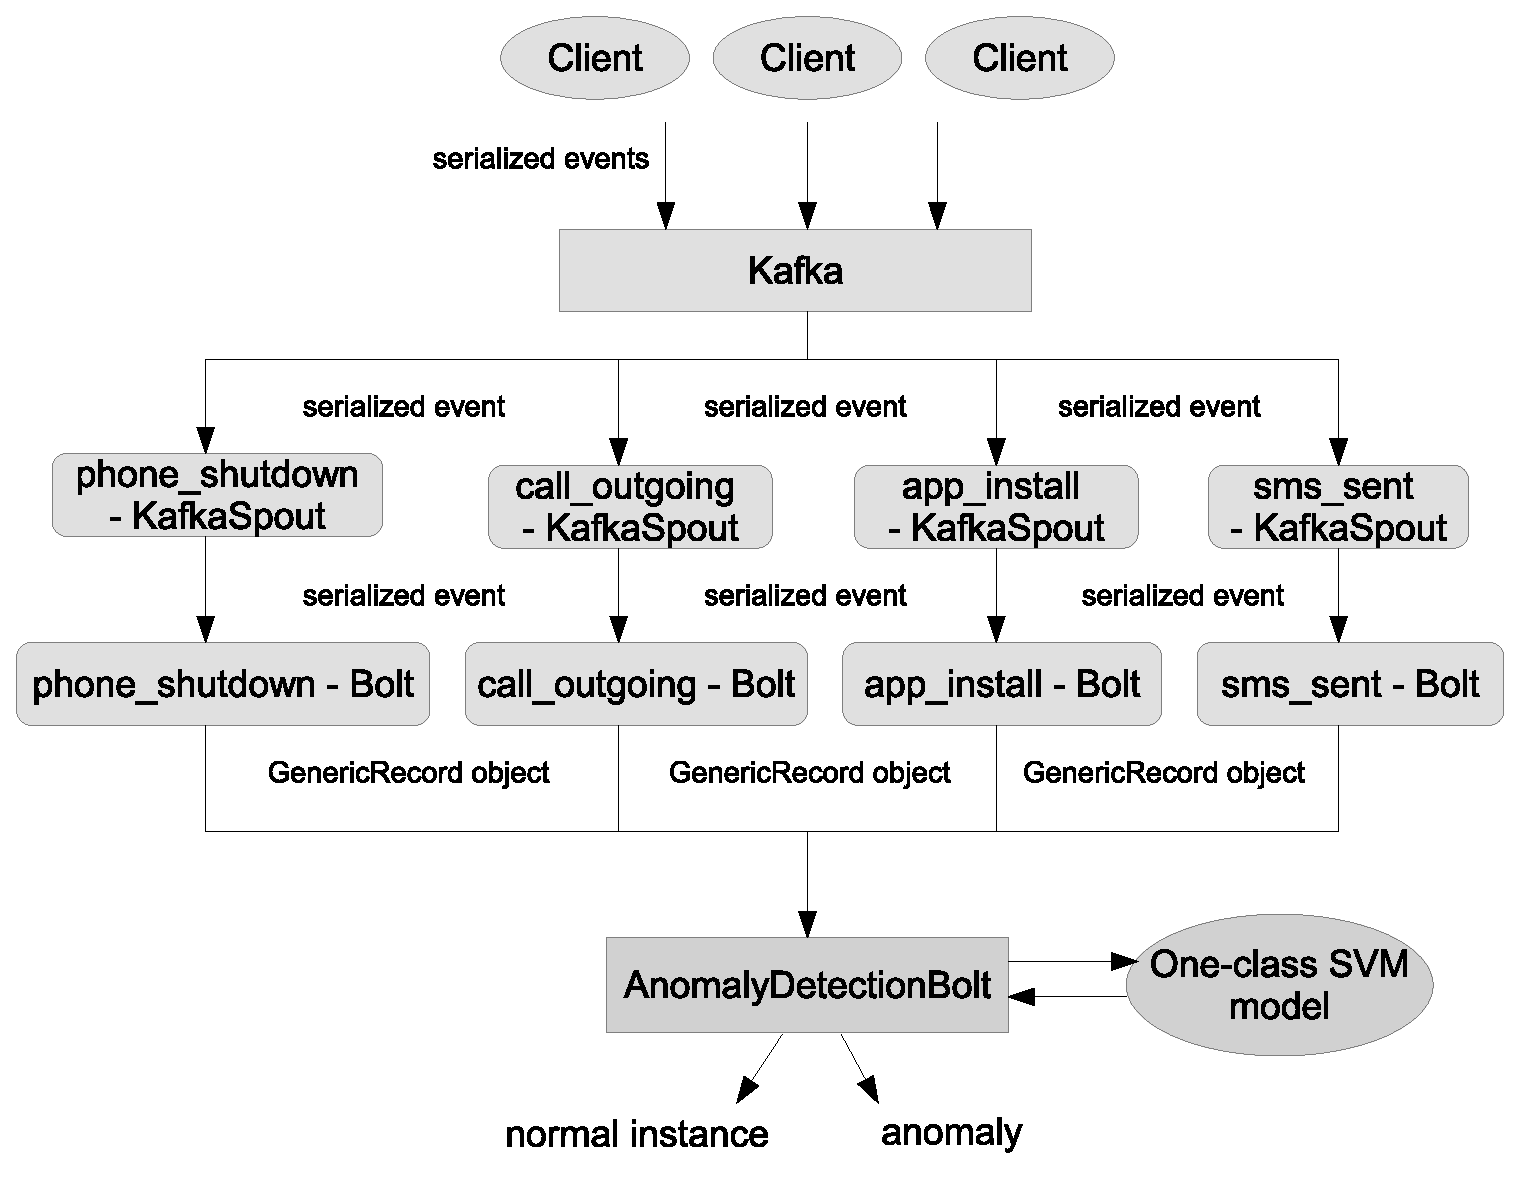
\includegraphics [width=1.0\textwidth]{images/anomaly_detection_data_flow}
  \caption{Anomaly detection: data flow}
  \label{fig:anomaly_detection_data_flow}
\end{figure}

For each Kafka topic a separate KafkaSpout receives messages.
One message contains the description of a particular event that happened on the client side (e.g. sms\_sent).
For each event type a separate bolt receives data from a corresponding KafkaSpout.
Then the bolt deserializes the received message, creating a \textit{GenericRecord} that represents the event.
For the events that are interesting for anomaly detection, there is an additional step.
Bolts, that receive data of type \textit{sms\_sent}, \textit{app\_install}, \textit{phone\_shutdown} and \textit{call\_outgoing}, emit the created GenericRecords to an \textit{AnomalyDetectionBolt}.

\mnote{Anomaly Detection bolt}
The main function of AnomalyDetectionBolt is to form data instances from incoming events.
As our version of Speed layer uses Redis as a data store, AnomalyDetectionBolt also uses it to accumulate events.
When a new event is received, AnomalyDetectionBolt extracts a type of event, a user id, and time when this event occured.
Using the user id, the bolt requests the value of \textit{lastCheckTime} that is stored in Redis.
The \textit{lastCheckTime} value is compared with the time, extracted from the received event.
If the time delta is bigger than a specified threshold, the new check for anomaly is performed.
The frequency of anomaly checks is regulated by an ANOMALY\_CHECK\_INTERVAL parameter.
This mechanism sets only one-side bound, so the check is performed not more than every half an hour by default.
However, if the bolt rare receives events from a particular user, the check for anomaly is run with the same low frequency. 

AnomalyDetectionBolt uses a sliding window to accumulate events.
The size of the window is regulated by a TTL parameter.
TTL specifies how long the event is stored in Redis.
Each time the new check for anomaly is performed, the bolt first of all deletes all outdated events from the store.
This guarantees that the data instance that participate in anomaly detection contains events that are collected over a specified period.
For example, the size of the sliding window is one hour by default.
If we want to perform an anomaly detection analysis, we take the mentioned earlier four types of events and count how many times each of them has occured during the last hour.
Using this numbers the bolt forms a data instance.  
Then it checks whether the instance is an anomaly or not using the trained one-class SVM model.

To get correct results it is essential to select the optimal parameters for One-class SVM.
Figure~\ref{fig:svm_parameters} represents the parameters, their meaning and values that are optimal for our case.
The process of parameters selection includes a technique called \textit{cross-validation}.
Here the data set is divided into two parts - training set and testing set.
This helps to avoid the problem of model overfitting.  

\begin{figure}[h]
  \centering
  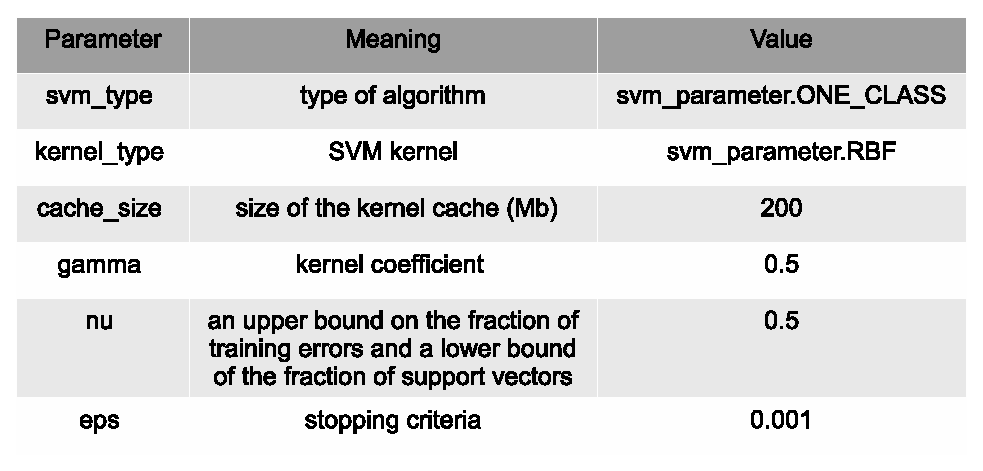
\includegraphics [width=0.9\textwidth]{images/svm_parameters}
  \caption{One-class SVM parameters}
  \label{fig:svm_parameters}
\end{figure}







 	

 
 
